\chapterOrPart{Formatting guidelines}\label{ch:formatting}
Your report or thesis will most probably contain elements such as figures, tables, numbers, units, symbols, mathematical expressions, citations and a bibliography. This chapter contains some guidelines and good practices for the proper formatting of these elements.

\section{Figures}\label{sec:formatfigures}
Figures are visual representations such as drawings, schemes, photos, charts and graphs. Every figure must be referenced in your text, preferably before the figure appears. Some important aspects of a figure are shown in \cref{fig:demofigure} and are discussed below.

\begin{frame}{A figure also requires a clear and well-written caption}
    \begin{figure}\centering
    	    \begin{tikzpicture}[scale=0.8]\node at (0,0) [above right] {\includegraphics[width=0.9\linewidth]{figs/demofigure}};
    			%\draw [help lines] (0,0) grid (14,7); % uncomment to show grid
    			\draw [pin] (8.0,4.0)   |- + (0.5,1) node [right,align=left] {a good-quality figure};
    			\draw [pin] (0.9,1.0)   |- + (0.5,4.7) node [right,align=left] {a numbered identifier under the figure,\\referenced in the text};
    			\draw [pin] ( 2.7,0.6)  -| + (0,   -1) node [below,align=left] {a caption describing: the \textit{what}};
    			\draw [pin] (9.5 ,0.6)  -- + (0,   -1) node [below,align=left] {the \textit{so what}};
    			\draw [pin] (15.3 ,0.6) -- + (0,   -1) node [below,align=left] {the source};
			\end{tikzpicture}
    	\caption{Some important aspects of a figure and its caption}\label{fig:demofigure}
    \end{figure}
\end{frame}

First of all, your figure must be of good quality, which means that careful consideration must be given to graphical excellence and integrity (e.g. resolution, data-ink ratio, lie-factor, legend,\dots). See the excellent work of \textcite{tufte2001} and \textcite{doumont2009} for more information on these topics.

Secondly, your figure must have an unique identifier and a descriptive caption. The identifier is typically the word \textit{Figure} followed by a number. For a short report, these numbers are typically the counting numbers 1, 2, 3, etc. For a thesis or book with different chapters, the numbering of figures restarts at 1 at the beginning of each new chapter, but the chapter number is included in the figure number. See for example the number 4.7 in \cref{fig:demofigure}, which means that this is the seventh figure in chapter 4. The automatic assigning of figure numbers in \LaTeX\ is taken care of by the \verb|\caption| command. If you want the caption to appear under the figure, you must place the \verb|\caption| command on the last line in the figure environment. You can inspect the source code of \cref{fig:demofigure} to verify this.

A descriptive caption is a stand-alone text that must provide enough information to understand the figure, without consulting the text. The first word of the caption should be capitalized. The caption should contain a \textit{what} part and, if possible, a \textit{so what} part. The \textit{what} part clearly explains what is shown on the figure. Try to precise and complete, it's better to have a longer caption than a short incomplete or unclear caption. The \textit{so what} part is a statement and explains what the reader should pay attention to and/or contains a justification for showing the picture.

If you did not make the figure yourself, you must add the reference to the source of the figure at the end of your caption, preceded for instance by the word \verb|source:| If the figure came from an external source but was adapted by you, you can precede the reference to the source by \verb|adapted from:|

\section{Tables}\label{sec:formattables}
Tables are used to present data in a orderly manner. They can contain different kind of elements such as text, numbers and mathematical symbols and expressions. Every table must be referenced in your text, preferably before it appears. Some important aspects of a table are shown in \cref{tab:demotable} and are discussed below.

\begin{table}[htbp]\centering
  	\caption{Some important aspects of a table and its caption}\label{tab:demotable}
    \begin{tikzpicture}[scale=0.8]\node at (0,0) [above right] {\includegraphics[width=0.9\linewidth]{figs/demotable}};
		%\draw [help lines] (0,0) grid (14,7); % uncomment to show grid
		\draw [pin] (0.4,5.8)   |- + (0.5,2)    node [right,align=left] {a numbered identifier above the table,\\referenced in the text};
		\draw [pin] (2.3,4.65)  -| + (-1,0)     node [left,align=left] {a top border};
		\draw [pin] (2.3,4.3)   -| + (-1,-0.6)  node [left,align=left] {column headers};
		\draw [pin] (3,3.9)   -| + (-1.2,-1.5)  node [left,align=left] {some space};
		\draw [pin] (2.3,0.3)   -| + (-1,0)     node [left,align=left] {a bottom border};
		\draw [pin] (2.3,1.5)   -| + (-0.5,0)   node [left,align=left] {a good-quality table};
	    \draw [pin] (2.4,5.8)   |- + (0.5,0.75) node [right,align=left] {a caption describing: the \textit{what}};
		\draw [pin] (11.5,5.8)  |- + (0.5,0.75) node [right,align=left] {the \textit{so what}};
		\draw [pin] (7 ,5.1)    -| + (7.5, -2)  node [below,align=left] {the source};
		\draw [pin] ( 2.8,0.4)  -| + (0,   -1)  node [below,align=left] {column alignment: left};
		\draw [pin] ( 7.8 ,0.4) -- + (0,   -1)  node [below right,align=left] {left};
		\draw [pin] (10.3 ,0.4) -- + (0,   -1)  node [below left,align=right] {right};
		\draw [pin] (10.9 ,0.4) -- + (0,   -1)  node [below right,align=left] {left};
		\draw [pin] (12.1 ,0.4) -- + (0,   -1)  node [below right,align=left] {left};
	\end{tikzpicture}
\end{table}

First of all, your table must be of good quality and should provide clarity on the presented data. This means that careful consideration must be given to graphical excellence and integrity (e.g. readability, data formatting and alignment, data-ink ratio, legend,\dots).

Secondly, your table must have an unique identifier and a descriptive caption. The identifier is typically the word \textit{Table} followed by a number. For a short report, these are typically ordinal numbers such as 1, 2, 3, etc. For a thesis or book with different chapters, the numbering of tables restarts at 1 at the beginning of each new chapter, but the chapter number is included in the table number. Table 3.2 for example refers to the second table in chapter 3. The automatic assigning of table numbers in \LaTeX\ is taken care of by the \verb|\caption| command. If you want the caption to appear above the table, you must place it on the first line in the figure environment. You can inspect the source code of \cref{tab:demotable} to verify this. In Microsoft Word, captions should be added via the \texttt{insert caption} menu command.

A descriptive caption is a stand-alone text that must provide enough information to understand the data in the table, without the need to consult to text. The first word of the caption should be capitalised. The caption should contain a \textit{what} part and, if possible, a \textit{so what} part. The \textit{what} part clearly explains what is shown in the table. Try to precise and complete, it's better to have a longer caption than a short incomplete or unclear caption. The \textit{so what} part is a statement and explains what the reader should pay attention to and/or contains a justification for showing the table.

If you did not obtain the data in the table yourself, you must add the reference to the source of the data at the end of your caption, preceded for instance by the word \verb|source:|

If the table came from an external source but was adapted by you, you can precede the reference to the source by \verb|adapted from:|

\subsection{Column alignment}
The data in the columns should be aligned. Since we read from left to right, it is best to left-align columns (column type \texttt{l} in \LaTeX). This is especially true for text. Columns that contain numbers are an exception. They should be right-aligned (column type \texttt{r}) or aligned at the decimal separator (column type \texttt{S}). This makes it easier to compare numbers in the same column. Columns with symbols and columns with units can be centred (column type \texttt{c}), but they are easier to read when they are left-aligned.

\subsection{Horizontal and vertical lines}
Having too many horizontal and/or vertical lines in a table is considered as visual noise and is distracting to the eye. It also lowers the data-ink ratio. Most of the time, two horizontal lines will do, one at the top of the table (\verb|\toprule| command) and another at the bottom (\verb|\bottomrule| command) as in \cref{tab:demotable}. These lines visually separate the data in the table from the main text. The column headers are separated from the data by some extra space. This separation can also be achieved with a horizontal line (\verb|\midrule| command). Vertical lines are most of the time not required but can be added in some occasions to improve readability.

Compare for instance \cref{tab:demo1} and \cref{tab:demo2}. Both tables contain exactly the same data but \cref{tab:demo2} has the better data-ink ratio and is therefore recommended.

\begin{table}\centering
    \caption{Dummy table with unnecessary horizontal and vertical lines, giving rise to a low data-ink ratio}\label{tab:demo1}
    \begin{tabular}{|l|r|l|l|} 
        \hline
         parameter  &  value & unit         & comment\\[1.5ex]    
         \hline
         voltage    &  12   & \si{\volt}    & given\\
         \hline
         current    &  2    & \si{\ampere}  & given\\
         \hline
        power       &  24   & \si{\watt}    & calculated\\
        \hline
    \end{tabular}
\end{table}

\begin{table}\centering
    \caption{Dummy table with a top and a bottom line only, giving rise to a higher data-ink ratio}\label{tab:demo2}
    \begin{tabular}{lrll}  
        \toprule
         parameter  &  value & unit         & comment\\[1ex]
         voltage    &  12   & \si{\volt}    & given\\
         current    &  2    & \si{\ampere}  & given\\
        power       &  24   & \si{\watt}    & calculated\\
        \bottomrule
    \end{tabular}
\end{table}

\section{Symbols}\label{sec:formatsymbols}
\subsection{Use of symbols}
Symbols are typically used to represent \emph{physical properties} and the units they are expressed in. Physical properties play an important role in physics and engineering. Well-known physical properties are for example the mass, temperature, velocity, pressure and electric current, but there are many others.

Physical quantities can be scalars (e.g. the mass $m$ and temperature $T$) but they can also be vectors (e.g. the force $\vec{F}$ and the velocity $\vec{V}$) or tensors.

The value of a scalar physical quantity is expressed with a number and an associated unit. One can say, for example: the ambient temperature is 298~kelvin. Note that both the name of the physical quantity (ambient temperature) and the name of the unit (kelvin) were written in full. That is perfectly acceptable but not so practical to use in calculations and formulas. That is why we often switch to a compact notation with \emph{symbols}.

For example, one can rewrite the statement regarding the ambient temperature as follows: the ambient temperature $ T_\up{environment}$ is 298~kelvin. Note that we used the symbol $T$ for the temperature. This is merely an agreement and  other symbols for the temperature are also possible. For example, other reference works sometimes use the symbol $\theta$ for the temperature. It is therefore advisable to always consult the symbol list or nomenclature of a scientific publication to find out which symbols were used.

Useful information about the physical quantity can be mentioned in the subscript; in this example the fact that it concerns the temperature of the environment). So $_\up{environment}$ was added as a subscript to the symbol $T$.

There are also symbols for units. For example, the symbol for the kelvin is the uppercase letter K. The above statement concerning the ambient temperature can be rewritten as follows: the ambient temperature $T_\up{environment}$ is \SI{298}{\kelvin}.

\subsection{Formatting of symbols}
One-letter symbols that represent (physical) quantities -- such as for example the temperature $T$ and the voltage $U$ -- are written in italics. Everything else is written upright, as illustrated in the flowchart in \cref{fig:italics}.  Symbols that consist of more than one letter -- such as for instance the Mach number (Ma) or the Net Present Values (NPV) -- are written upright, otherwise they might be mistaken as products. That's why for instance the Reynolds number is written as Re and not as $Re$, because that could be interpreted as the product of the radius $R$ with the eccentricity $e$.

The fact that many symbols must be written upright will give you some kind of struggle, because in the math mode of \LaTeX\, letters are written in italics by default, unless you manually force them upright. The same is true for the Equation editor of Microsoft Word, there too, the standard way of writing is in italics. But no worries, how to deal with this and how to get things right is explained below.

\begin{frame}{Only one-letter symbols that represent quantities are written in italics}
    \begin{figure}\centering
        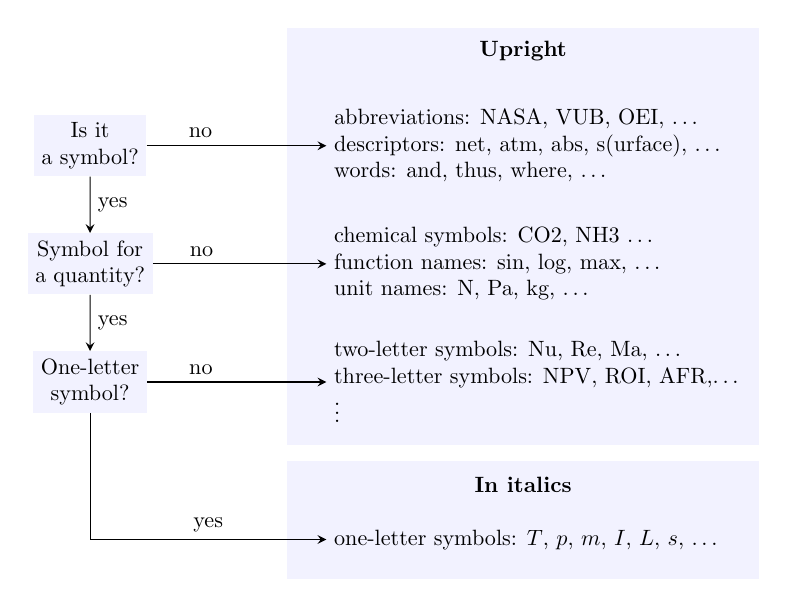
\begin{tikzpicture}[node distance=2cm,every node/.style={scale=0.8}]
            \tikzstyle{examples} = [rectangle, anchor=west,align=left]
            %\tikzstyle{decision} = [rectangle ,align=center,fill=blue!05]
            \tikzstyle{decision} = [rectangle ,align=center,fill=blue!05]
            \tikzstyle{arrow} = [thin,->,>=stealth]
            \tikzstyle{description} = [font=\bfseries]
            \tikzstyle{descriptionbox} = [fill=blue!05,align=left,right]
            %\draw [helpline] (0,0) grid (12,8);
        
            \node (symbol) [decision] at (3,5) {Is it\\ a symbol?};
            \node (quantity) [decision] at (3,3.5) {Symbol for\\ a quantity?};
            \node (oneletter) [decision] at (3,2) {One-letter\\ symbol?};
            
            \fill[descriptionbox] (5.5,1.2) rectangle (11.5,6.5);
            \fill[descriptionbox] (5.5,-0.5) rectangle (11.5,1);
            \node [description] at (8.5,6.2)  {Upright};
            \node [description] at (8.5,0.7)  {In italics};
            
            \node (nosymbol) [examples] at (6,5) {
            abbreviations: NASA, VUB, OEI, \dots\\
            descriptors: net, atm, abs, s(urface), \dots\\
            words: and, thus, where, \dots};
            
            \node (noquantity) [examples] at (6,3.5) {
            chemical symbols: \ch{CO2}, \ch{NH3} \dots\\
            function names: sin, log, max, \dots\\
            unit names: N, Pa, kg, \dots};
            
            \node (nooneletter) [examples] at (6,2) {
            two-letter symbols: Nu, Re, Ma, \dots\\
            three-letter symbols: NPV, ROI, AFR,\dots\\
            $\vdots$};
            
            \node (yesoneletter) [examples] at (6,0) {
            one-letter symbols: $T$, $p$, $m$, $I$, $L$, $s$, \dots};
            
            \draw [arrow] (symbol)   -- node[right] {yes}  (quantity);
            \draw [arrow] (quantity) -- node[right] {yes} (oneletter);
            \draw [arrow] (oneletter) |- node[above,pos=0.75] {yes} (yesoneletter);
            \draw [arrow] (symbol) -- node[above,pos=0.3] {no} (nosymbol);
            \draw [arrow] (quantity) -- node[above,pos=0.28] {no} (noquantity);
            \draw [arrow] (oneletter) -- node[above,pos=0.3] {no} (nooneletter);
        \end{tikzpicture}
        \caption{Flowchart to determine if something must be written upright or in italics: only one-letter symbols for quantities must be written in italics}\label{fig:italics}
    \end{figure}
\end{frame}

Some examples are given below and in \cref{tab:up}. So, as already mentioned, only one-letter symbols for quantities are written in italics:
\begin{align*}
    \text{correct:} \quad & T = \SI{298}{\kelvin} \\
    \text{not correct:} \quad & \up{T} = \SI{298}{\kelvin}
\end{align*}

The same goes for one-letter symbols that appear in subscripts and superscripts. The subscript $p$ for example in the specific heat capacity $c_{p}$ is written in italics because it represents a quantity:
\begin{align*}
    \text{correct:} \quad & c_{p} \quad \text{(because $p$ is a symbol for a quantity)} \\
    \text{not correct:} \quad & c_\up{p} \\
    \text{correct:} \quad & p_\up{gauge} = p_\up{abs} - p_\up{atm}\quad \text{(because the subscripts are not symbols for quantities)} \\
    \text{not correct:} \quad & p_{gauge} = p_{abs} - p_{atm}
\end{align*}

Natural constants are also quantities and their one-letter symbols are therefore also written in italics, as for example, the universal gas constant\footnote{the u in the subscript is written upright because it is not a symbol for a quantity, it's just the first letter of the word 'universal'} $R_\up{u}$ or the speed of light in vacuum $c$. 

\begin{frame}[fragile]{Some stuff is always written upright}\scriptsizebeamer
    \begin{table}\centering
    \caption{Some things are always written upright}\label{tab:up}
        \begin{tabular}{llll}
        \toprule
        type & examples & a \LaTeX\ example & \LaTeX\ result  \\[+1.5ex]
        %\midrule
        descriptions & abs, net, \dots & \verb|$p_\up{atm}$| & $p_\up{atm}$\\
        symbols for units & Pa, kg, \dots & \verb|\si{m^2}| & \si{\square\meter}\\% see package siunitx
        math functions & log, max, \dots & \verb|$\sin\alpha$| & $\sin\alpha$\\
        chemical formulas & \ch{NH3}, \ch{CO2}, \dots & \verb|\ch{CH4}| & $\ch{CH4}$\\ % see package chemformula
        multi-letter symbols & Ma, Nu, \dots & \verb|$\up{Re}=2300$| & $\up{Re}=2300$\\
        acronyms and abbreviations & NPV, NASA, \dots & \verb|$\up{AFR}= 50$| & $\up{AFR}= 50$\\
        \bottomrule
        \end{tabular}
    \end{table}
\end{frame}

More-letter symbols for quantities are written upright:
\begin{align*}
    \text{correct:}     \quad & \up{Ma} = 0.80 \\
    \text{not correct:} \quad & Ma = 0.80 \quad \text{(undesired spacing + looks like $M$ times $a$)}\\
    \text{correct:}     \quad & \text{NPV = 3000~\euro} \\
    \text{not correct:} \quad & NPV = \text{3000~\euro} \quad \text{(undesired spacing + looks like $N$ times $P$ times $V$)}
\end{align*}

Descriptions are written upright:
\begin{align*}
    \text{correct:} \quad & T_\up{environment} = \SI{298}{\kelvin} \\
    \text{not correct:} \quad & T_{environment} = \SI{298}{\kelvin}
\end{align*}

Even if you shorten the descriptive text to make the notation more compact, you still write it upright:
\begin{align*}
    \text{correct:} \quad & T_\up{env} = \SI{298}{\kelvin} \\
    \text{not correct:} \quad & T_{env} = \SI{298}{\kelvin}
\end{align*}

Even descriptions reduced to a single letter are written upright:
\begin{align*}
    \text{correct:} \quad & T_\up{e} = \SI{298}{\kelvin}\quad \text{(because e is not a symbol for a quantity)} \\
    \text{not correct:} \quad & T_{e} = \SI{298}{\kelvin}
\end{align*}

Words are written upright, even when they appear between mathematical expressions:
\begin{align*}
    \text{correct:}     \quad &  U=I R \quad \text{with the current} \quad I=\SI{2}{\ampere}\\
    \text{not correct:} \quad &  U=I R \quad and\ the\ current \quad I=\SI{2}{\ampere}
\end{align*}

Words are written upright, even when they appear in mathematical expressions:
\begin{align*}
    \text{correct:}     \quad &   \eta=\frac{\text{work produced}}{\text{heat received}}\\
    \\
    \text{not correct:} \quad &   \eta=\frac{work\ produced}{heat\ received}
\end{align*}

Symbols for mathematical functions are written upright:
\begin{align*}
    \text{correct:}     \quad &   \sin\alpha\\
    \text{not correct:} \quad &   sin\alpha
\end{align*}

Chemical formulas are written upright:
\begin{align*}
    \text{correct:}     \quad &   \ch{CO2}\\
    \text{not correct:} \quad &       CO_2
\end{align*}

\section{Numbers}\label{sec:formatnumbers}
\subsection{Decimal separator}
In Belgium it is customary to use the comma as the decimal separator (e.g. $\pi\approx$ 3,14), while in the English scientific literature the dot is used ($\pi\approx$ 3.14). 

It is important that you consistently use the same decimal separator throughout your document, otherwise the reader will get confused. If you include figures/tables from English-language literature (that contain numbers with the dot as decimal separator), it is advised to use the dot as the decimal separator for your entire document.

\subsection{Thousands separator}
It is good practise to separate the thousands in a number with a small non-breakable space. This makes a number with many digits easier to read. The \verb|siunitx| package can take care of that, see \cref{sec:siunitx} for more info.

For instance the command \verb|\num{1000000}| produces \num{1000000}. 

The use of the comma as a thousands separator is to be avoided, this to avoid confusion for people in Belgium who are used to the comma as a decimal separator.

\subsection{Significant digits}
It is good practice to write only the significant digits of a number, because a too large number of decimal digits creates a false impression of precision. For instance, a value of 123.456789876~m for a measured length with a simple ruler probably contains decimal digits that are not meaningful. Are you sure up to the level of millimeters, then you can write the number as \SI{123.456}{\meter}. Are you only sure of three significant digits, then you write \SI{123}{\meter}.

If the number of significant digits is lower than the number of digits before the decimal separator, it is better to use a prefix or switch to exponential notation. Are you for example only sure of the first two digits in \SI{123}{\meter}, then you can rewrite it as \SI{0.012}{km} or \SI{1.2E2}{meter}.

\section{Units}\label{sec:formatunits}
Except for dimensionless quantities, numbers without units make no sense. Units are always written upright, never in italics:
\begin{align*}
    \text{correct:} \quad & L = \SI{7}{meter} \\
    \text{not correct:} \quad & L = 7 \; meter
\end{align*}

Symbols for units, like the letter m for meter, are also written upright:
\begin{align*}
    \text{correct:} \quad & L = \SI{7}{\meter} \\
    \text{not correct:} \quad & L = 7 \; m
\end{align*}

In this way there can be no confusion between the symbol $m$ that is used for mass and the symbol m that is used for meter. And so, for example, $A$ represents an area in \si{\square\meter} and the A written upright represents the unit ampere for electric current.

Do not use abbreviations for units. Use the symbol or the full name:
\begin{align*}
    \text{correct:} \quad & \text{s or second; m/s or meters per second} \\
    \text{not correct:} \quad & \text{sec, mps}
\end{align*}

The symbol used for a unit is never written in the plural form:
\begin{align*}
    \text{correct:} \quad & z = \SI{120}{\centi\meter}\\
    \text{not correct:} \quad & z = 120 \; \up{cms}
\end{align*}

No full stop is put after a unit, unless that unit is at the end of a sentence:
\begin{align*}
    \text{correct:} \quad & \text{The length of the tube is 70~cm.}\\
    \text{correct:} \quad & \text{The tube is 70~cm long.} \\
    \text{not correct:} \quad & \text{The tube is 70~cm. long.}
\end{align*}

Prefixes representing a multiplication factor (\cref{t:factors}) are also written upright and written together with the symbol of the unit
\begin{align*}
    \text{correct:} \quad & \pres_\up{1} = \SI{700}{\kilo\pascal} \\
    \text{not correct:} \quad & \pres_\up{1} = 700 \, \up{k \, Pa}
\end{align*}

\begin{table}\centering
\caption{Some standard prefixes in SI units}\label{t:factors}
    \begin{tabular}{llll}
        \toprule
        factor & prefix & factor & prefix \\[+1.5ex]
        \num{E-1}  & deci  &  \num{E1}  & deca \\
        \num{E-2}  & centi &  \num{E2}  & hecto \\
        \num{E-3}  & milli &  \num{E3}  & kilo \\
        \num{E-6}  & micro &  \num{E6}  & mega \\
        \num{E-9}  & nano  &  \num{E9}  & giga \\
        \num{E-12} & pico  &  \num{E12} & terra \\
        \num{E-15} & femto &  \num{E15} & peta \\
        \bottomrule
    \end{tabular}
\end{table}

\subsection{Spaces}
A number must be kept together with its unit. This can be achieved by putting an unbreakable space between the number and the unit. This will 'glue' the unit to the number, so that the number doesn't end up alone at the end of a line with the unit at the start of the next line.

To achieve this in \LaTeX\ you use the tilde \verb|~| in text mode and the \verb|\;| in math mode. So for instance \verb|80~kg| will appear as 80~kg. Or even better, you can use the package \verb|siunitx| that will take care of the proper spacing for you.

In Microsoft Word you must type \textsc{shift-ctrl-space} to produce an unbreakable space.

The unit can also be 'glued' to the number by suppressing the space between them, but this is considered as bad practice.
\begin{align*}
    \text{correct:} \quad & \vol =\SI{3}{\cubic\meter} \\
    \text{bad practice:} \quad & \vol = 3 \up{m ^ 3}
\end{align*}

\section{Mathematical expressions}\label{sec:formatmath}
\subsection{Equations}
It is good practice to number your equations, because it allows to cross-reference them from elsewhere in your text. Automatic numbering can be achieved by using the \texttt{equation} environment, as shown in the first law of thermodynamics for closed systems below
\begin{equation}\label{eq:1stlawclosedsystem}
    \Delta E = Q + W.
\end{equation}

To establish a cross-reference, you must first add a label to the equation environment. You can then use this label in a \verb|\cref{...}| command elsewhere. Inspect the source code of \cref{eq:1stlawclosedsystem} to see how this is done.

There are many other math-environments available in \LaTeX\ that can do more complicated things with equations such as splitting, grouping and aligning. More info is available on the Overleaf help page about \href{https://www.overleaf.com/learn/latex/Aligning_equations_with_amsmath}{aligning equations with amsmath}.

\subsection{Multiplication sign}
To write a multiplication of two variables, leave a small space between them or put a proper multiplication operator between them. In math-mode in \LaTeX, use \verb|\cdot| to produce the center dot $\cdot$ or use \verb|\times| to produce the multiplication sign $\times$.

In Microsoft Word, you can use \verb|\bullet| in the equation editor to produce the center dot $\cdot$.

Other symbols, such as the asterisk *, the letter x and the full stop, should be avoided.
\begin{frame}[fragile]{Some good and bad symbols for multiplying}
    \begin{align*}
    \text{correct:} \quad & U = I\, R \\
    \text{correct:} \quad & U = I\cdot R\\
    \text{correct:} \quad & U = I\times R \\
    \text{not recommended:} \quad & U = I * R \\
    \text{bad practice:} \quad & U = I x R \\
    \text{bad practice:} \quad & U = I.R
    \end{align*}
\end{frame}

\subsection{Punctuation}
Equations are part of the sentence structure, which means
punctuation must be respected. See the example below.

Newton's second law is
\begin{equation}\label{eq:newton}
    \vec{F} = m \cdot \vec{a},
\end{equation}
where $\vec{F}$  is the force,  $m$ the mass and $\vec{a}$ the acceleration.




\section{Using other people's work}\label{sec:formatcites}
In your report or thesis you will probably use information from other sources. If you do so, you have to explain to the reader where this information came from and where this information can be found. This is of great importance for the following three reasons:
\begin{enumerate}
    \item it gives proper credit to the authors or creators of your sources
    \item it allows the reader of your work to look-up and consult the source to learn more about a subject
    \item it avoids that you are being suspected of plagiarism
\end{enumerate}

\subsection{Citing}
Citing is the crediting of author(s) of a source, directly in your text. This is done by putting in-text citations in the body of your text. They are typically placed immediately after the information being cited. In \LaTeX\ we use the package \texttt{BibLaTeX} to take care of the citations, see \cref{sec:biblatex} for more info. There are three commands you should know when citing.

The \verb|\cite| command is used to refer to the work itself, as part of the sentence. For example:

\begin{quotation}
The visual display of quantitative information is discussed in \cite{tufte2001}.
\end{quotation}

The \verb|\textcite| command is used to refer to the author(s) of the work, as part of the sentence.
\begin{quotation}
 \textcite{tufte2001} discusses how quantitative information is visually displayed.
\end{quotation}

The \verb|\parencite| command is used to cite the work when the sentence is already complete. In such a case, the citation is just placed between parentheses at the end of the sentence, but before the full stop!
\begin{quotation}
 Quantitative information is visually displayed in different ways \parencite{tufte2001}.
\end{quotation}

There are many different citation styles, see \cref{tab:cites} with three popular citation styles (author-year, numeric and alphabetic) and the effect on the three cite commands discussed above.

\subsection{Sources}
You should use reliable sources, such as articles from scientific journals. Wikipedia for instance, can certainly be useful as inspiration, and help you understand certain things better, but can't be regarded as primary scientific source material. It's better to consult and use the underlying sources that Wikipedia is citing. So in principle, no reference to Wikipedia should appear in your reference list. But of course exceptions are possible.

\subsection{The bibliography}
The bibliography is a list with all the cited sources in your work. It is typically placed at the very end of your document. It must contain the necessary information to find back the references. Typically: the names of the authors, the title of the work, the publication date, details of the publisher and the book/journal.

In this template, the command \verb|\printbibliography| at the end of the main file produces the bibliography. There are many different styles for a bibliography but we advise you to use one of the standard styles. As was already the case with the citations, the package \texttt{BibLaTeX} will take care of the bibliography. See \cref{sec:biblatex} for more info on this package.

\section{English}\label{sec:formatenglish}
In the European Union, British English is mostly used. American English can also be used, if there are reasons to do so. In any case, you should consistently use one type of spelling throughout your entire document, so American and British spelling cannot be mixed. Some examples of the differences between the British and American spelling are shown in \cref{tab:english}.

\begin{table}[b]\centering
	 \caption{Some examples of words in British and American spelling; in the EU, British English is recommended}\label{tab:english}
        \begin{tabular}{ll}
            \toprule
             British        & American\\[+1.5ex]
             analyse        & analyze\\
             aerofoil       & airfoil\\
             aeroplane      & airplane\\
             behaviour      & behavior\\
             centre         & center\\
             colour         & color\\
             defence        & defense\\
             labelled       & labeled\\
             litre          & liter\\
             metre          & meter\\
             modelling      & modeling\\
             modelled       & modeled\\
             mould          & mold\\
             neighbour      & neighbor\\
             programme      & program\\
             vapour         & vapor\\
             \bottomrule
        \end{tabular}
\end{table}

\mode<all> 
% Required because of the \mode* command at the beginning of this file.
% See beameruserfile.pdf section 21.3 for more info











